Before the proofs that are the main results of this thesis we will start with a formal introduction of partizan poset games in general and partizan poset games played on chess-colored Young diagrams in particular.
%\\
\begin{defn}[Partizan Poset Games]
Let $P$ be any colored poset and let $p_L,p_R$ denote arbitrary elements in $P$ of Left and Right respectively. The partizan poset game $G_{\rm PP}(P)$ played on $P$ is a partizan two-player game where the Left player has the option to select any white element $p_L$ in $P$ and then remove $p_L$ together with all elements greater than $p_L$ and equivalently for the Right player but with black elements in $P$. More formally we have:
\begin{align*}
&G_{\rm PP}(P)=\{L|R\}&~\\
&L=\{G_{\rm PP}(P\setminus S_{\rm P}(p_L)):p_L\in P\text{ is white}\}&~\\
&R=\{G_{\rm PP}(P\setminus S_{\rm P}(p_R)):p_R\in P\text{ is black}\}&\\
&S_{\rm P}(p)=\{p':p'\in P,p'\ge p\}&~
\end{align*}
\end{defn}
~\\
More specifically, this thesis deals with partizan poset games played on posets that are chess-colored and in the form of Young diagrams. We will denote such a game, with $k\ge1$ rows in the Young diagram, as $A_\lambda$, where $\lambda=(\lambda_1,\lambda_2,\dots,\lambda_k)$ is as in Definition \ref{def:lambda} and $\lambda_1\ge \lambda_2\ge \dots\ge \lambda_k$ denotes the lengths of the 1st, 2nd,$\dots,k$'th rows respectively. In particular, when $k=3$ or $k=2$, we will use the notation $A_{x,y,z}$ and $A_{x,y}$ respectively.

\subsection{All Poset Games Are Numbers}
As it is, we have that all poset games are numbers. In particular, for a large number of partizan poset games, the value is bounded.% as $0\le G\le 1$.
%According to Section \ref{section:numbers} in general and Theorem \ref{numthm} in particular, it is, using \emph{Conway Induction}, sufficient to show that for a poset game $G$ we have $G^L<G^R$.
%\\
\begin{thm}
\label{thm:posetnum}
All poset games are numbers.
\end{thm}
\begin{proof2}{Proof of Theorem \ref{thm:posetnum}}
Assume that we have an arbitrary poset game $G$. Using \emph{Conway Induction} (Theorem \ref{thm:conind}) it suffices to assume that $G^L,G^R$ are numbers and then deduce that $G$ is a number as well. By Theorem \ref{thm:number} it is then sufficient to show that $G^L<G^R$ for all options of $G$.
\\
If we can show that $G^L<G$ and $G^R>G$ for any Left and Right options of $G$, then it also holds that $G^L<G^R$, and hence $G$ must be a number.
\\\\
Consider the scenario where Left moves to some option $G^{L_1}$, as illustrated in Figure \ref{fig:posetnum1}. We have that $G^{L_1}<G$ since Right always wins in $G^{L_1}-G$.
\\
\begin{figure}[H]
\centering
\begin{subfigure}{0.45\textwidth}
\begin{tikzpicture}
\path[draw,use Hobby shortcut,closed=true]
(0,-0.2) .. (1.2,1) .. (2.5,2) .. (.3,3.3) .. (-1.4,1.3) .. (-1.3,.3);
\node (G) at (0.3,1.5) {$G$};
\end{tikzpicture}
\end{subfigure}
%$\hfill$
\begin{subfigure}{0.45\textwidth}
\begin{tikzpicture}
\path[draw,use Hobby shortcut,closed=true]
(0,0) .. (.5,1) .. (1,2) .. (.3,3) .. (-1,1) .. (-1,.5);
\path[dashed,draw,use Hobby shortcut,closed=true]
(0,-0.2) .. (1.2,1) .. (2.5,2) .. (.3,3.3) .. (-1.4,1.3) .. (-1.3,.3);
\path[draw,use Hobby shortcut,closed=true]
(1.5,2.3) .. (1.8,2) .. (2,2.4) .. (1.7,3);
\node (G) at (0,1.5) {$G^{L_1}$};
\draw (1,2) -- (1.5,2.3);
\node at (1.5,2.3) {\tikz\draw[black,fill=white] (0,0) circle (.5ex);};
\draw [<-,thick] (1.5,1) -- (2,0.5);
\node at (2.2,.3) {G};
\end{tikzpicture}
\end{subfigure}
\captionof{figure}{Arbitrary poset game $G$ and $G$ with an arbitrary Left option $G^{L_1}$.}
\label{fig:posetnum1}
\end{figure} 

This is easily understood from the following. In the game $G^{L_1}-G$ in Figure \ref{fig:posetnum2} the Right player wins if it plays first, since then Right can move to $-G^{L_1}$ in $-G$ and then mimic Left's moves until Left has no moves left. If Left starts and plays in the part of $G$ that is not included in $G^{L_1}$, i.e., the small appendage of G in Figure \ref{fig:posetnum1}, then Right can move to $-G^{L_1}$ in that component and copy Left in the same way as before. If Left starts and plays in the $G^{L_1}$-part of either component, then Right can copy Left until either Left has no moves or until Left plays in the appendage part of the $-G$ component, and then Right can just move to the option that removes that appendage, which makes the two components mirrored again, so Right can then copy Left until Left has no moves and loses.
\\
Since Right wins in $G^{L_1}-G$ no matter if Right starts or not, then $G^{L_1}-G<0$.
\begin{figure}[H]
\centering
\begin{tikzpicture}
\path[draw,use Hobby shortcut,closed=true]
(0,0) .. (.5,1) .. (1,2) .. (.3,3) .. (-1,1) .. (-1,.5);
\node (G) at (0,1.5) {$G^{L_1}$};
\end{tikzpicture}
{\scalefont{10}
\begin{tikzpicture}
\node at (0,3){};
\node at (0,1.5){-};
\node at (0,0){};
\end{tikzpicture}
}
\begin{tikzpicture}
\path[draw,use Hobby shortcut,closed=true]
(0,0) .. (.5,1) .. (1,2) .. (.3,3) .. (-1,1) .. (-1,.5);
\path[dashed,draw,use Hobby shortcut,closed=true]
(0,-0.2) .. (1.2,1) .. (2.5,2) .. (.3,3.3) .. (-1.4,1.3) .. (-1.3,.3);
\path[draw,use Hobby shortcut,closed=true]
(1.5,2.3) .. (1.8,2) .. (2,2.4) .. (1.7,3);
\node (G) at (0,1.5) {$G^{L_1}$};
\draw (1,2) -- (1.5,2.3);
\node at (1.5,2.3) {\tikz\draw[black,fill=white] (0,0) circle (.5ex);};
\end{tikzpicture}
\captionof{figure}{The poset game $G^{L_1}-G$.}
\label{fig:posetnum2}
\end{figure}
%\\
In the exact same way, it is possible to show that Left always wins in $G^{R_1}-G$, and hence that $G^{R_1}-G>0$. We therefore have $G^{L_1}<G^{R_1}$. Since $G^{L_1}$ and $G^{R_1}$ were arbitrary, this holds for any Left and Right options $G^{L_1},G^{R_1}$, and therefore $G$ must be a number.
\end{proof2}

This lets us know that all poset games are numbers. But we can also bound the value of some partizan poset games, as will be seen in Theorem \ref{thm:value}.

\begin{minipage}[b]{0.5\textwidth}
\begin{thm}
Any partizan poset game $G$ with a single smallest element colored white, covered only by black elements, has a value $0< G< 1$. 
\\
An example game can be seen in Figure \ref{fig:partizanvalue}.
\label{thm:value}
\end{thm}
\end{minipage}
\begin{minipage}{0.05\textwidth}
~
\end{minipage}
\begin{minipage}[b]{0.45\textwidth}

%\begin{figure}[H]
\centering
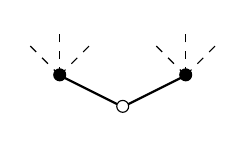
\begin{tikzpicture}[baseline=-0.65ex,scale=.2]
  \draw[thick] (0,-2) -- (-4,0);
  \draw[thick] (0,-2) -- (4,0);
  \draw[dashed] (-4,0) -- (-6,2);
  \draw[dashed] (-4,0) -- (-4,3);
  \draw[dashed] (-4,0) -- (-2,2);
  \draw[dashed] (4,0) -- (6,2);
  \draw[dashed] (4,0) -- (4,3);
  \draw[dashed] (4,0) -- (2,2);
  \node (zero) at (0,-2) {\tikz\draw[black,fill=white] (0,0) circle (.5ex);};
  \node (1) at (-4,0) {\tikz\draw[black,fill=black] (0,0) circle (.5ex);};
  \node (2) at (4,0) {\tikz\draw[black,fill=black] (0,0) circle (.5ex);};
\end{tikzpicture}
\captionof{figure}{}
\label{fig:partizanvalue}
%\end{figure}
\end{minipage}
\begin{proof2}{Proof of Theorem \ref{thm:value}}
Let $G$ be any partizan poset game with a single smallest element colored white, covered only by black elements. Clearly $G>0$ since Left can remove the smallest element in the poset, removing all elements, resulting in no options for Right, so Left wins. 
\\
Moreover, since the game with only the smallest (white) element left is either an option of Right, or an option of an option of Right, or an option of an option of an option of Right,\dots, etc., and all $G^R>G$, then $G<1$.
\end{proof2}
%Obviously, the value of games for which the coloring is reversed that of Theorem \ref{thm:value} is also bounded, but as $0>G>-1$ instead. 
%\\
We may note that this theorem holds for all chess-colored partizan poset games with a single smallest elements, e.g., games played on chess-colored Young diagrams.
\\\\
In addition to bounding the value of some games, it is also possible to determine that a player should try to play the option of removing as great elements as possible.
\begin{thm}[Play Strategy]
\label{thm:playstrategy}
A player should only play the options of removing elements not lower than any other element of the same color.
\end{thm}
\begin{proof2}{Proof of Theorem \ref{thm:playstrategy}}
We will prove this theorem by showing that any option of removing an element that is lower than some other element of the same color is also a dominated option. 
\\
Let $G$ be any partizan poset game, let $G^{L_{x_1}},G^{L_{x_2}}$ be the Left options when removing the elements $x_1$ and $x_2$ respectively and let $x_1>x_2$.
The option $G^{L_{x_2}}$ must be an option of $G^{L_{x_1}}$. This is because $x_1>x_2$, which yields that the option of removing $x_2$ also removes $x_1$, and therefore the option of removing $x_1$ does not remove any elements that are not removed when playing the option of removing $x_2$. 
\\
Since $G^{L_{x_2}}$ is an option of $G^{L_{x_1}}$ and Theorem \ref{thm:posetnum} yields that $G$ is a number, then $G^{L_{x_1}}>G^{L_{x_2}}$ and hence $G^{L_{x_2}}$ is dominated by $G^{L_{x_1}}$, i.e., Left should not play the option $G^{L_{x_2}}$.
\\
Similarly, this holds for Right options as well.
\end{proof2}
\newpage
%
%\subsection{Partizan Tree Poset Games And Blue-Red Hackenbush}
%\begin{thm}
%A Partizan tree poset game where no element is covering more than one element is equivalent to a game of Blue-Red Hackenbush.
%\end{thm}
%\begin{proof2}
%Consider a partizan tree poset game $G$. Then transform every element in the poset of $G$ to a stick in the game of Blue-Red Hackenbush, color them according to the appropriate player, connect every stick with the stick that it covers and connect the least element to the ground. We then have an equivalent game of Blue-Red Hackenbush.
%\begin{figure}[H]
%\centering
%\begin{tikzpicture}[scale=1]
%  \node (zero) at (-6,-1) {\tikz\draw[black,fill=white] (0,0) circle (.5ex);};
%  \node (1) at (-8,.5) {\tikz\draw[black,fill=black] (0,0) circle (.5ex);};
%  \node (2) at (-6,.5) {\tikz\draw[black,fill=white] (0,0) circle (.5ex);};
%  \node (3) at (-4,.5) {\tikz\draw[black,fill=black] (0,0) circle (.5ex);};
%  \node (4) at (-9,2) {\tikz\draw[black,fill=black] (0,0) circle (.5ex);};
%  \node (5) at (-7,2) {\tikz\draw[black,fill=white] (0,0) circle (.5ex);};
%  \node (6) at (-4,2) {\tikz\draw[black,fill=white] (0,0) circle (.5ex);};
%  \draw[thick] (zero) -- (1) -- (4);
%  \draw[thick] (zero) -- (2);
%  \draw[thick] (1) -- (5);
%  \draw[thick] (zero) -- (3) -- (6);
%%\end{tikzpicture}
%%\begin{tikzpicture}[scale=0.5]
%    \draw[densely dashed] (-1,-1) -- (1,-1);
%    \node[hackennode] (down)   at ( 0,  -1) {};
%    \node[hackennode] (middle) at ( 0,   0) {};
%    \node[hackennode] (left)   at (-1.5, 1) {};
%    \node[hackennode] (right)  at ( 1.5, 1) {};
%    \node[hackennode] (top)    at ( 0,   1) {};
%    \node[hackennode] (top2)   at (-2,   2) {};
%    \node[hackennode] (top3)   at (-1,   2) {};
%    \node[hackennode] (top4)   at ( 1.5, 2) {};
%
%    \draw[hackenline,blue]
%		(down) -- (middle);
%    \draw[hackenline,red]
%		(middle) -- (right);
%    \draw[hackenline,red]
%		(middle) -- (left);
%    \draw[hackenline,blue]
%        (middle) -- (top);
%    \draw[hackenline,red]
%        (left) -- (top2);
%    \draw[hackenline,blue]
%        (left) -- (top3);
%    \draw[hackenline,blue]
%        (right) -- (top4);
%
%\end{tikzpicture}
%\end{figure}
%\begin{figure}[H]
%\centering
%\begin{tikzpicture}[scale=1]
%  \node (zero) at (-6,-1) {\tikz\draw[black,fill=white] (0,0) circle (.5ex);};
%  \node (1) at (-8,.5) {\tikz\draw[black,fill=black] (0,0) circle (.5ex);};
%  \node (2) at (-6,.5) {\tikz\draw[black,fill=white] (0,0) circle (.5ex);};
%  \node (3) at (-4,.5) {\tikz\draw[black,fill=black] (0,0) circle (.5ex);};
%  \node (4) at (-9,2) {\tikz\draw[black,fill=black] (0,0) circle (.5ex);};
%  \node (5) at (-7,2) {\tikz\draw[black,fill=white] (0,0) circle (.5ex);};
%  \node (6) at (-4,2) {\tikz\draw[black,fill=white] (0,0) circle (.5ex);};
%  \draw[thick] (zero) -- (1) -- (4);
%  \draw[thick] (zero) -- (2);
%  \draw[thick] (1) -- (5);
%  \draw[thick] (zero) -- (3) -- (6);
%%\end{tikzpicture}
%%\begin{tikzpicture}[scale=0.5]
%    \draw[densely dashed] (-1,-1) -- (1,-1);
%    \node[hackennode] (down)   at ( 0,  -1) {};
%    \node[hackennode] (middle) at ( 0,   0) {};
%    \node[hackennode] (left)   at (-1.5, 1) {};
%    \node[hackennode] (right)  at ( 1.5, 1) {};
%    \node[hackennode] (top)    at ( 0,   1) {};
%    \node[hackennode] (top2)   at (-2,   2) {};
%    \node[hackennode] (top3)   at (-1,   2) {};
%    \node[hackennode] (top4)   at ( 1.5, 2) {};
%
%    \draw[hackenline,blue]
%		(down) -- (middle);
%    \draw[hackenline,red]
%		(middle) -- (right);
%    \draw[hackenline,red]
%		(middle) -- (left);
%    \draw[hackenline,blue]
%        (middle) -- (top);
%    \draw[hackenline,red]
%        (left) -- (top2);
%    \draw[hackenline,blue]
%        (left) -- (top3);
%    \draw[hackenline,blue]
%        (right) -- (top4);
%
%\draw[<->, blue, shorten <= 0.25cm, shorten >= 0.1cm] (-6,-1) to[out=-20,in=-180] (0,-.5);
%\draw[<->, red, shorten <= 0.25cm, shorten >= 0.1cm] (-8,.5) to[out=20,in=-135] (-.625,.25);
%\draw[<->, blue, shorten <= 0.25cm, shorten >= 0.1cm] (-6,.5) to[out=-30,in=-180] (0,.5);
%\draw[<->, red, shorten <= 0.25cm, shorten >= 0.1cm] (-4,.5) to[out=50,in=140] (.875,.75);
%\draw[<->, red, shorten <= 0.25cm, shorten >= 0.1cm] (-9,2) to[out=30,in=-160] (-1.75,1.5);
%\draw[<->, blue, shorten <= 0.25cm, shorten >= 0.1cm] (-7,2) to[out=30,in=120] (-1.1,1.8);
%\draw[<->, blue, shorten <= 0.25cm, shorten >= 0.1cm] (-4,2) to[out=30,in=160] (1.5,1.5);
%
%
%\end{tikzpicture}
%\end{figure}
%\begin{figure}[H]
%\centering
%\begin{tikzpicture}[scale=1]
%    \draw[densely dashed] (-1,-1) -- (1,-1);
%    \node[hackennode] (down)   at ( 0,  -1) {};
%    \node[hackennode] (middle) at ( 0,   0) {};
%    \node[hackennode] (left)   at (-1.5, 1) {};
%    \node[hackennode] (right)  at ( 1.5, 1) {};
%    \node[hackennode] (top)    at ( 0,   1) {};
%    \node[hackennode] (top2)   at (-2,   2) {};
%    \node[hackennode] (top3)   at (-1,   2) {};
%    \node[hackennode] (top4)   at ( 1.5, 2) {};
%
%    \draw[hackenline,blue]
%		(down) -- (middle);
%    \draw[hackenline,red]
%		(middle) -- (right);
%    \draw[hackenline,red]
%		(middle) -- (left);
%    \draw[hackenline,blue]
%        (middle) -- (top);
%    \draw[hackenline,red]
%        (left) -- (top2);
%    \draw[hackenline,blue]
%        (left) -- (top3);
%    \draw[hackenline,blue]
%        (right) -- (top4);
%        
%  \node (zero) at (0,-.5) {\tikz\draw[black,fill=white] (0,0) circle (1ex);};
%  \node (1) at (-.75,.5) {\tikz\draw[black,fill=black] (0,0) circle (1ex);};
%  \node (2) at (-0,.5) {\tikz\draw[black,fill=white] (0,0) circle (1ex);};
%  \node (3) at (.75,.5) {\tikz\draw[black,fill=black] (0,0) circle (1ex);};
%  \node (4) at (-1.75,1.5) {\tikz\draw[black,fill=black] (0,0) circle (1ex);};
%  \node (5) at (-1.25,1.5) {\tikz\draw[black,fill=white] (0,0) circle (1ex);};
%  \node (6) at (1.5,1.5) {\tikz\draw[black,fill=white] (0,0) circle (1ex);};
%%  \draw[thick, dashed] (zero) -- (1) -- (4);
%%  \draw[thick, dashed] (zero) -- (2);
%%  \draw[thick, dashed] (1) -- (5);
%%  \draw[thick, dashed] (zero) -- (3) -- (6);
%\end{tikzpicture}
%\end{figure}
%jjjj
%\end{proof2}
%\newpage

\subsection{Chess-Colored Young Diagram Partizan Poset Games}
For chess-colored Young diagrams, we have a very regular structure. This regularity makes it possible to reduce the games significantly, and make even stronger statements about the values of these games. A general result about how we can reduce games played on chess-colored Young diagrams is the following.

\begin{lem}
\label{lem:chessdomopt}
The dominating option of $A_\lambda$, with $\lambda=(\lambda_1,\lambda_2,\dots,\lambda_k)$, is always to remove the greatest element of your color in one of the rows.
\end{lem}
~\\
Lemma \ref{lem:chessdomopt} follows from Theorem \ref{thm:playstrategy}. For a better understanding of what the lemma yields, we will provide some examples of the concept. 
\begin{ex}{}
Let $k=4$. With $\lambda_1=9,\lambda_2=7,\lambda_3=7,\lambda_4=2$, Lemma \ref{lem:chessdomopt} gives us that: $$A_{9,7,7,2}=\left\{A_{8,7,7,2},A_{9,5,5,2},A_{9,7,6,2},A_{9,7,7,1}\middle|A_{7,7,7,2},A_{9,6,6,2},A_{9,7,5,2},A_{9,7,7,0}\right\}.$$
\end{ex}
\begin{ex}{}
For $x=y=3,z=1$ Lemma \ref{lem:chessdomopt} gives us $$A_{3,3,1}=\left\{A_{2,2,1},A_{3,1,1},A_{3,3,0}\middle|A_{1,1,1},A_{3,2,1}\right\},$$ as illustrated in Figure \ref{fig:chessdomex}.
\begin{figure}[H]
\centering
$
\begin{tabular}{ | c | c | c |}
\hline
~&\cellcolor[gray]{0}&~\\
\hline
\cellcolor[gray]{0}&~&\cellcolor[gray]{0}\\
\hline
~\\
\cline{1-1}
\end{tabular}
=\left\{
\begin{tabular}{ | c | c |}
\hline
~&\cellcolor[gray]{0}\\
\hline
\cellcolor[gray]{0}&~\\
\hline
~\\
\cline{1-1}
\end{tabular}
,
\begin{tabular}{ | c | c | c |}
\hline
~&\cellcolor[gray]{0}&~\\
\hline
\cellcolor[gray]{0}\\
\cline{1-1}
~\\
\cline{1-1}
\end{tabular}
,
\begin{tabular}{ | c | c | c |}
\hline
~&\cellcolor[gray]{0}&~\\
\hline
\cellcolor[gray]{0}&~&\cellcolor[gray]{0}\\
\hline
\end{tabular}
\;\middle|\;
\begin{tabular}{ | c |}
\hline
~\\
\hline
\cellcolor[gray]{0}\\
\hline
~\\
\hline
\end{tabular}
,
\begin{tabular}{ | c | c | c |}
\hline
~&\cellcolor[gray]{0}&~\\
\hline
\cellcolor[gray]{0}&~\\
\cline{1-2}
~\\
\cline{1-1}
\end{tabular}
\right\}
$
\captionof{figure}{Concept of Lemma \ref{lem:chessdomopt}.}
\label{fig:chessdomex}
\end{figure}
\end{ex}
%~\\
%Lemma \ref{lem:chessdomopt} follows from Theorem \ref{thm:playstrategy}, but we will provide an explicit proof and prove Lemma \ref{lem:chessdomopt} using Theorem \ref{thm:number} by showing that options when removing non-maximal elements are options of a option when a maximal element is removed, and must therefore be dominated by this option. 
%\begin{proof2}{Proof of Lemma \ref{lem:chessdomopt}}
%Let $G=A_\lambda$, with $\lambda=(\lambda_1,\lambda_2,\dots,\lambda_k)$, and let $G^{L_i},i\in\{1,2,\dots,k\}$ denote an arbitrary option of Left when playing in the $i$'th row and $G^{R_i},i\in\{1,2,\dots,k\}$ denote an arbitrary option of Right when playing in the $i$'th row. Let $G^{L_i^{max}},G^{R_i^{max}}$ denote the game options of $G$ when removing the greatest white and black element respectively in the $i$'th row for players Left and Right. \\
%We will then have that $G^{L_i^{max}}>G^{L_i}$ for any other option for Left in the $i$'th row. This is because any other Left option when playing in the $i$'th row except removing the greatest Left element is a game option of $G^{L_i^{max}}$ and by Theorem \ref{thm:number} we have $G^{L_i^{max}L}<G^{L_i^{max}}$. The same argument also gives us that $G^{R_i^{max}}<G^{R_i}$ for all other Right options of playing in the $i$'th row. Therefore $G^{L_1^{max}},G^{L_2^{max}},G^{L_3^{max}}, G^{R_1^{max}},G^{R_2^{max}},G^{R_3^{max}}$ must be the dominating game options of $G$, and hence Lemma \ref{lem:chessdomopt} is valid for $G$ itself.
%\end{proof2}

\newpage
\subsubsection{Two-Row Chess-Colored Young Diagrams}
In this section we will prove that a partizan poset game played on a chess-colored two-row Young diagram is easy to compute by providing a formula to compute any such game $A_{x,y}$.
\begin{thm}
\label{thm:2rowvalue}
There is a formula, given by (\ref{eq:2rowvalue}), to compute the value of partizan poset games played on chess-colored two-row Young diagrams.
\begin{equation}
\label{eq:2rowvalue}
A_{x,y}=
\frac{2}{5}+\frac{1}{15}2^{-(2y-2)}(-1)^y-\frac{1}{3}2^{-(x+y-1)}(-1)^x
\end{equation}
\end{thm}
This is proved by using Lemma \ref{lem:chessdomopt} to reduce the game $A_{x,y}$ to two options per player, and, inductively, using the formula to determine which option is dominating to reduce the game to one option per player. Then, using Theorem \ref{thm:number}, it is just a matter of showing that the formula in fact yields the simplest number between the two dominating options.
\begin{proof2}{Proof of Theorem \ref{thm:2rowvalue}}
Assume that Theorem \ref{thm:2rowvalue} is true for all options of a game $A_{x,y}$. We will then show that the theorem then also holds for the game itself. By Conway Induction, this yields that Theorem \ref{thm:2rowvalue} is true.
From Lemma \ref{lem:chessdomopt} we have that the dominating options of $A_{x,y}$ are to remove the greatest possible element in one of the rows. 
\\
Assume $x\ge y+2,y\ge2$. This yields that $A_{x-2,y},A_{x-1,y},A_{x,y-1},A_{x,y-2}$ are the dominating options of $A_{x,y}$. We want to find out when which options are dominating. We do that by comparing the differences between the values of the options using (\ref{eq:2rowvalue}), to see which is greater and when.
\\
If $x$ and $y$ are both even, then $A_{x,y}=\left\{ A_{x-2,y},A_{x,y-1}\middle|A_{x-1,y},A_{x,y-2}\right\}$. This yields the following differences between the option values:
\begin{align*}
\begin{split}
A_{x-2,y}-A_{x,y-1}&=2^{-(2y-2)}(-1)^y\frac{1}{3}\Bigl(1-(-2)^{-(x-y)}\Bigr)\\
&\ge0\text{ if $x\ge y$ and $y$ is even}\\
&\le0\text{ if $x\ge y$ and $y$ is odd}
\end{split}\\
\begin{split}
A_{x-1,y}-A_{x,y-2}&=2^{-(2y-2)}(-1)^y\Bigl(-1+(-2)^{-(x-y)}\Bigr)\\
&\ge0\text{ if $x\ge y$ and $y$ is odd}\\
&\le0\text{ if $x\ge y$ and $y$ is even}
\end{split}
\end{align*}
Since $x\ge y$, clearly $A_{x-2,y}$ dominates $A_{x,y-1}$ for Left and $A_{x-1,y}$ dominates $A_{x,y-2}$ for Right, and hence $A_{x,y}=\left\{A_{x-2,y}\middle|A_{x-1,y}\right\}$ if $x$ and $y$ are even.
\\
Similarly, if $x$ and $y$ are both odd, then $A_{x,y}=\left\{A_{x-1,y},A_{x,y-2}\middle|A_{x-2,y},A_{x,y-1}\right\}$, and from the equations above, we have that $A_{x-1,y}$ dominates $A_{x,y-2}$ for Left and $A_{x-2,y}$ dominates $A_{x,y-1}$ for Right. Hence $A_{x,y}=\left\{A_{x-1,y}\middle|A_{x-2,y}\right\}$ if $x$ and $y$ are odd.
\\
For the other combination of parities of $x$ and $y$, we have the following value differences:
\begin{align*}
\begin{split}
A_{x-2,y}-A_{x,y-2}&=(-4)^{-(y-1)}\\
&>0\text{ if $y$ is odd}\\
&<0\text{ if $y$ is even}
\end{split}\\
\begin{split}
A_{x-1,y}-A_{x,y-1}&=2^{-(2y-2)}(-1)^y\frac{1}{3}\left(1+2(-2)^{-(x-y)}\right)\\
&\ge0\text{ if $x\ge y$ and $y$ is even}\\
&\le0\text{ if $x\ge y$ and $y$ is odd}
\end{split}
\end{align*}
Clearly, $A_{x-2,y},A_{x,y-1}$ are options of Left (Right) only if $x,y$ are even (odd), and $A_{x-1,y},A_{x,y-2}$ are options of Left (Right) only if $x,y$ are odd (even). This yields that $A_{x-2,y},A_{x-1,y}$ always dominate $A_{x,y-1},A_{x,y-2}$, given that $x\ge y+2$. 
\\
In other words, if $x\ge y+2$, 
\begin{align*}
A_{x,y}=\left\{
\begin{array}{l l}
\left\{A_{x-2,y}\middle|A_{x-1,y}\right\}&\text{ if $x$ is even,}\\
~\\
\left\{A_{x-1,y}\middle|A_{x-2,y}\right\}&\text{ if $x$ is odd.}
\end{array}\right.
\end{align*}
Using Theorem \ref{thm:number}, we therefore only need to show that the value of $A_{x,y}$ given by (\ref{eq:2rowvalue}) is the same as the simplest number in between the options above. If we compare the dominating options by examining the difference between their values, and the proposed value of the game, we get:
\begin{equation}
\begin{split}
A_{x-2,y}-A_{x-1,y}&=2^{-(x+y-1)}\left(-2(-1)^x\right)\\
A_{x-2,y}-A_{x,y}&=2^{-(x+y-1)}\left(-(-1)^x\right)\\
A_{x,y}-A_{x-1,y}&=2^{-(x+y-1)}\left(-(-1)^x\right)
\end{split}\tag{*}
\label{eq:2simpldiff}
\end{equation}
In other words we can see that the absolute difference in the numerator between the option values is 2, and that the proposed value is the only value with the same denominator in between the value of the options. From Definition \ref{def:simpnum} we can conclude that the proposed value for $A_{x,y}$ in fact is the simplest number between the options, and hence that Equation (\ref{eq:2rowvalue}) holds for $x\ge y+2,y\ge2$.
\\
Now, assume $x\ge y+2,y=1$. We can then reduce $A_{x,y}$ to:
\begin{align*}
A_{x,y}=\left\{
\begin{array}{l l}
\left\{A_{x-2,1}\middle|A_{x-1,1},A_{x,0}\right\}&\text{ if $x$ is even}\\
~\\
\left\{A_{x-1,1}\middle|A_{x-2,1},A_{x,0}\right\}&\text{ if $x$ is odd}
\end{array}\right.
\end{align*}
If we compare the value yields the value differences:
\begin{align*}
\begin{split}
A_{x-1,1}-A_{x,0}&=\frac{1}{3}\left(-1+(-2)^{-(x-2)}\right)\\
&\le0\text{ if $x\ge2$ is even}
\end{split}\\
\begin{split}
A_{x-2,1}-A_{x,0}&=\frac{1}{3}\left(-1+(-2)^{-(x-1)}\right)\\
&\le0\text{ if $x\ge 1$}
\end{split}
\end{align*}
As we can see, playing in the first row always dominates playing in the second row for Right if $x\ge y+2,y=1$. In other words, we have the game
\begin{align*}
A_{x,y}=\left\{
\begin{array}{l l}
\left\{A_{x-2,1}\middle|A_{x-1,1}\right\}&\text{ if $x$ is even,}\\
~\\
\left\{A_{x-1,1}\middle|A_{x-2,1}\right\}&\text{ if $x$ is odd.}
\end{array}\right.
\end{align*}
Comparing these options with the proposed game value yields the same results as in (\ref{eq:2simpldiff}), but substituted with $y=1$, and hence (\ref{eq:2rowvalue}) holds for $x\ge y+2,y=1$ as well.
\\
Now, assume $x\ge y+2,y=0$. Then
\begin{align*}
A_{x,y}=\left\{
\begin{array}{l l}
\left\{A_{x-2,0}\middle|A_{x-1,0}\right\}&\text{ if $x$ is even,}\\
~\\
\left\{A_{x-1,0}\middle|A_{x-2,0}\right\}&\text{ if $x$ is odd.}
\end{array}\right.
\end{align*}
As with $y=1$, comparing the values of these options with the proposed game value yields the same results as in (\ref{eq:2simpldiff}), but substituted with $y=0$, and hence (\ref{eq:2rowvalue}) holds for $x\ge y+2,y=0$ as well. 
\\
We can therefore conclude that (\ref{eq:2rowvalue}) holds for $x\ge y+2,y\ge0$. 
\\
Now, assume $x=y+1,y\ge2$.We then have the following game:
\begin{align*}
A_{x,y}=A_{y+1,y}=\left\{
\begin{array}{l l}
\left\{A_{y,y},A_{y+1,y-1}\middle|A_{y-1,y-1},A_{y+1,y-2}\right\}&\text{ if $y$ is even}\\
~\\
\left\{A_{y-1,y-1},A_{y+1,y-2}\middle|A_{y,y},A_{y+1,y-1}\right\}&\text{ if $y$ is odd}
\end{array}\right.
\end{align*} 
Comparing the options yields the differences:
\begin{align*}
\begin{split}
A_{y,y}-A_{y+1,y-1}&=0
\end{split}\\
\begin{split}
A_{y-1,y-1}-A_{y+1,y-2}&=(-4)^{-(y-1)}\\
&>0\text{ if $y$ is odd}\\
&<0\text{ if $y$ is even}
\end{split}
\end{align*}
As $A_{y-1,y-1},A_{y+1,y-2}$ are options of Left (Right) only if $y$ is odd (even), clearly $A_{y-1,y-1}$ dominates over $A_{y+1,y-2}$. Moreover, since $A_{y,y}=A_{y+1,y-1}$, then they dominate each other, so we can choose to always play in the first row here as well. This lets us reduce the game to
\begin{align*}
A_{x,y}=A_{y+1,y}=\left\{
\begin{array}{l l}
\left\{A_{y,y}\middle|A_{y-1,y-1}\right\}&\text{ if $y$ is even,}\\
~\\
\left\{A_{y-1,y-1}\middle|A_{y,y}\right\}&\text{ if $y$ is odd.}
\end{array}\right.
\end{align*}
If we compare the values of the dominating options and the proposed game value the same way as before, we have:
\begin{equation*}
\begin{split}
A_{y,y}-A_{y-1,y-1}&=4^{-y}\left(-2(-1)^y\right)\\
A_{y,y}-A_{y+1,y}&=4^{-y}\left(-(-1)^y\right)\\
A_{y+1,y}-A_{y-1,y-1}&=4^{-y}\left(-(-1)^y\right)
\end{split}
\end{equation*}
As before, this yields that the proposed value of the game is the simplest number between its dominating options, and hence (\ref{eq:2rowvalue}) holds for $x=y+1,y\ge2$.
\\
Now, assume $x=y,y\ge2$. This yields the game
\begin{align*}
A_{x,y}=A_{y,y}=\left\{
\begin{array}{l l}
\left\{A_{y-2,y-2},A_{y,y-1}\middle|A_{y-1,y-1},A_{y,y-2}\right\}&\text{ if $y$ is even,}\\
~\\
\left\{A_{y-1,y-1},A_{y,y-2}\middle|A_{y-2,y-2},A_{y,y-1}\right\}&\text{ if $y$ is odd.}
\end{array}\right.
\end{align*}
Comparing the values of these options yields the differences:
\begin{align*}
\begin{split}
A_{y-2,y-2}-A_{y,y-1}&=(-4)^{-(y-1)}\\
&>0\text{ if $y$ is odd}\\
&<0\text{ if $y$ is even}
\end{split}\\
\begin{split}
A_{y-1,y-1}-A_{y,y-2}&=0
\end{split}
\end{align*}
As $A_{y-2,y-2},A_{y,y-1}$ are options of Left (Right) only if $y$ is even (odd), then clearly $A_{y,y-1}$ dominates over $A_{y-2,y-2}$, i.e., it is dominating to play in the second row. Since $A_{y-1,y-1}=A_{y,y-2}$, we can choose to always play in the second row here too. This yields the reduced game
\begin{align*}
A_{x,y}=A_{y,y}=\left\{
\begin{array}{l l}
\left\{A_{y,y-1}\middle|A_{y,y-2}\right\}&\text{ if $y$ is even,}\\
~\\
\left\{A_{y,y-2}\middle|A_{y,y-1}\right\}&\text{ if $y$ is odd.}
\end{array}\right.
\end{align*}
If we compare the values of these options and the proposed value of the game as before, we get:
\begin{equation*}
\begin{split}
A_{y,y-1}-A_{y,y-2}&=4^{-y}\left(-4(-1)^y\right)\\
A_{y,y-1}-A_{y,y}&=4^{-y}\left(-2(-1)^y\right)\\
A_{y,y}-A_{y,y-2}&=4^{-y}\left(-2(-1)^y\right)
\end{split}
\end{equation*}
In analogy with before, this yields that the proposed value of the game is the simplest number between its dominating options, and hence (\ref{eq:2rowvalue}) holds for $x=y,y\ge2$.
\\
Now, the only cases left are when $x< y+2,y<2$, a finite number of cases. It is therefore sufficient to check by hand if (\ref{eq:2rowvalue}) holds for these four cases. For these cases, i.e., $(x,y)\in\left\{(0,0),(1,1),(1,0),(2,1)\right\}$, we have, respectively, 
\begin{align*}
A_{0,0}&=\left\{\middle|\right\}=0\\
A_{1,1}&=\left\{A_{0,0}\middle|A_{1,0}\right\}=\left\{0\middle|1\right\}=\frac{1}{2},\\
A_{1,0}&=\left\{A_{0,0}\middle|\right\}=\left\{0\middle|\right\}=1,\\
A_{2,1}&=\left\{A_{0,0}\middle|A_{1,1},A_{2,0}\right\}=\left\{0\middle|\frac{1}{2},\frac{1}{2}\right\}=\frac{1}{4},
\end{align*} 
which are all equal to the formula proposed values.
\\
As we can see that (\ref{eq:2rowvalue}) also holds for these for cases, we can conclude that it also holds for $x< y+2,y<2$, which also yields that it holds for any $x\ge y,y\ge0$. 
\\
This completes the proof.
\end{proof2}
\newpage
\subsubsection{Three-Row Chess-Colored Young Diagrams}
In this section we will prove that a partizan poset game played on a chess-colored three-row Young diagram is easy to compute by providing and proving correctness of a formula to compute the value of any such game $A_{x,y,z}$.
%\\
\begin{thm}
\label{thm:3rowvalue}
There is a formula, with equations given by (\ref{eq:3rowvalue}), to compute the value of partizan poset games played on any chess-colored three-row Young diagrams. 
%\\
%In particular, we have that the value of $A_{x,y,z}$ is given by (\ref{eq:3row1}) if $x,y,z\ge4$, (\ref{eq:3row2}) if $x,y\ge4,z=3$, (\ref{eq:3row3}) if $x,y\ge4,z=2$, (\ref{eq:3row4}) if $x\ge4,y=3,z=3$, (\ref{eq:3row5}) if $x\ge4,y=3,z=2$, (\ref{eq:3row6}) if $x\ge4,y=2,z=2$, (\ref{eq:3row7}) if $x=y,y\ge 1,z=1$, (\ref{eq:3row8}) if $x=y+1,y\ge 1,z=1$, (\ref{eq:3row9}) if $x>y,y\ge1,z=1$, (\ref{eq:3row10}) if $x>y,y\ge1,z=1$, (\ref{eq:3row11}) if $z=0$, (\ref{eq:3row12}) if $x=2,y=2,z=2$, (\ref{eq:3row13}) if $x=3,y=2,z=2$, (\ref{eq:3row14}) if $x=3,y=3,z=2$, (\ref{eq:3row15}) if $x=3,y=3,z=3$.
\begin{subequations}
\label{eq:3rowvalue}
\begin{align}
\label{eq:3row1}
\begin{split}
\frac{237}{512} & -2^{-(2z+1)}\left(\frac{2^{z+1}}{3}\left((-1)^z-2^{z-4}\right)-\frac{1}{5}\left((-1)^z-4^{z-4}\right)\right)\\
& -2^{-(y+z+1)}\left(2^{z+1}-1\right)(-1)^y\frac{1}{3}\left(1-(-2)^{y-z}\right)\\
& -2^{-x}(-1)^x\frac{1}{3}\left(1-(-2)^{x-y}\right)\\
%&\text{ if $x\ge y\ge z\ge4$}
\end{split}%&\text{ if $x\ge y\ge z\ge4$}
&&x\ge y\ge z\ge4
\\
\label{eq:3row2}
\begin{split}
\frac{119}{256}&-2^{-(y+4)}(-1)^y5\left(1-(-2)^{y-4}\right)\\
& -2^{-x}(-1)^x\frac{1}{3}\left(1-(-2)^{x-y}\right)\\
%&\text{ if $x\ge y\ge4, z=3$}
\end{split}
&&x\ge y\ge 4,z=3
\\
\label{eq:3row3}
\begin{split}
\frac{59}{128}&-2^{-(y+3)}(-1)^y\frac{7}{3}\left(1-(-2)^{y-4}\right)\\
& -2^{-x}(-1)^x\frac{1}{3}\left(1-(-2)^{x-y}\right)\\
%&\text{ if $x\ge y\ge4, z=2$}
\end{split}
&&x\ge y\ge 4,z=2
\\
\label{eq:3row4}
\begin{split}
\frac{59}{128}&-2^{-x}(-1)^x\frac{1}{3}\left(1-(-2)^{x-4}\right)\\
%&\text{ if $x\ge 4,y=3,z=3$}
\end{split}
&&x\ge 4,y=z=3
\\
\label{eq:3row5}
\begin{split}
\frac{29}{64}&-2^{-x}(-1)^x\frac{1}{3}\left(1-(-2)^{x-4}\right)\\
%&\text{ if $x\ge 4,y=3,=2$}
\end{split}
&&x\ge 4,y=3,z=2
\\
\label{eq:3row6}
\begin{split}
\frac{15}{32}&-2^{-x}(-1)^x\frac{1}{3}\left(1-(-2)^{x-4}\right)\\
%&\text{ if $x\ge 4,y=2,z=2$}
\end{split}
&&x\ge 4,y=z=2
\\
\label{eq:3row7}
\begin{split}
\frac{1}{2}&-2^{-(y+3)}(-1)^y\left(3-(-1)^y\right)\\
%&\text{ if $x=y\ge z=1$}
\end{split}
&&x=y,z=1
\\
\label{eq:3row8}
\begin{split}
\frac{1}{2}&-2^{-(y+3)}(-1)^y\left(-3-(-1)^y\right)\\
%&\text{ if $x=y+1,y\ge z=1$}
\end{split}
&&x=y+1,z=1
\\
\label{eq:3row9}
\begin{split}
\frac{1}{2}&+\frac{1}{3}2^{-(y+1)}-\frac{1}{3}2^{-(x-1)}(-1)^x\\
%&\text{ if $x>y\ge z=1$ and $y$ is even}
\end{split}
&&
\begin{array}{l}
x>y\ge z=1\\
\text{and x is even}
\end{array}
\\
\label{eq:3row10}
\begin{split}
\frac{1}{2}&-\frac{1}{3}2^{-(y+2)}-\frac{1}{3}2^{-x}(-1)^x\\
%&\text{ if $x>y\ge z=1$ and $y$ is odd}
\end{split}
&&
\begin{array}{l}
x>y\ge z=1\\
\text{and x is odd}
\end{array}
\\
\label{eq:3row11}
\begin{split}
\frac{2}{5}&+\frac{1}{15}4^{-(y-1)}(-1)^y-\frac{1}{3}2^{-(x+y-1)}(-1)^x\\
%&2^{-(x+2y-1)}\left(\frac{2^x}{5}\Big(2^{2y}-(-1)^y\Big)+\frac{1}{3}\Big(2^x(-1)^y-2^y(-1)^x\Big)\right)\\
%&\text{ if $x\ge y\ge z=0$}
\end{split}
&&x\ge y\ge z=0
\\
\label{eq:3row15}
\begin{split}
\frac{35}{64}
\end{split}
&&x=y=z=3
\\
\label{eq:3row14}
\begin{split}
\frac{17}{32}
\end{split}
&&x=y=3,z=2
\\
\label{eq:3row13}
\begin{split}
\frac{9}{16}
\end{split}
&&x=3,y=z=2
\\
\label{eq:3row12}
\begin{split}
\frac{13}{32}
\end{split}
&&x=y=z=2
\end{align}
\end{subequations}
\end{thm}
~\\
We will prove the theorem by induction, assuming that it is true for any option of an arbitrary game $A_{x,y,z}$, and from this showing that it is then also true for the game itself. But first, we will prove a lemma that we will use in order to reduce the game by specifying when to play in which row.
\begin{lem}
Assuming Theorem \ref{thm:3rowvalue} is true for all options of the game $A_{x,y,z}$, then the following is true.
\begin{itemize}
\item[(i)]Playing the option to remove the greatest element in the first row of your color is the dominating option if $x\ge y+z+1$.
\item[(ii)]Playing the option to remove the greatest element in the second row of your color is the dominating option if $x<y+z+1$ and $y>z$.
\item[(iii)]Playing the option to remove the greatest element in the third row of your color is the dominating option if $x<y+z+1$ and $y=z$ and $z>2$.
\item[(iv)]If $x<y+z+1$ and $y=z=1$, playing the option to remove the (only) element in the third row is the dominating option for Left and playing the option to remove the (only) element in the second row is the dominating option for Right.
\item[(v)]If $x<y+z+1$ and $y=z=2$, playing the option to remove the (only) white element in the second row is the dominating option for Left and playing the option to remove the (only) black element in the third row is the dominating option for Right.
\end{itemize}
\label{lem:rowopt}

\end{lem}
~\\
We will provide a short example of the concept for a more intuitive understanding of Lemma \ref{lem:rowopt}:
\begin{ex}{}~\\
With $x=23,y=10,z=6$, Lemma \ref{lem:rowopt} gives us that $A_{23,10,6}=\left\{A_{22,10,6}\middle| A_{21,10,6}\right\},$ i.e., we play in the first row.
\\
With $x=11,y=10,z=6$, Lemma \ref{lem:rowopt} gives us that $A_{11,10,6}=\left\{A_{11,8,6}\middle| A_{11,9,6}\right\},$ i.e., we play in the second row.
\\
With $x=11,y=6,z=6$, Lemma \ref{lem:rowopt} gives us that $A_{11,6,6}=\left\{A_{11,6,4}\middle| A_{11,9,5}\right\},$ i.e., we play in the third row.
\\
With $x=5,y=2,z=2$, Lemma \ref{lem:rowopt} gives us that $A_{5,2,2}=\left\{A_{4,2,2}\middle| A_{3,2,2}\right\},$ i.e., we play in the first row.
\\
With $x=4,y=2,z=2$, Lemma \ref{lem:rowopt} gives us that $A_{4,2,2}=\left\{A_{4,1,1}\middle| A_{4,2,1}\right\},$ i.e., we play in the second row.
\end{ex}
\begin{proof2}{Proof of Lemma \ref{lem:rowopt}}
Assume Theorem \ref{thm:3rowvalue} holds for all options of a game $A_{x,y,z}$. By Lemma \ref{lem:chessdomopt}, we only need to look at the options when removing maximal elements.
\\
We will begin to show when it is better to play in the second and third row, independently of the first row.
\\
Assume $y=z$, we then have the following dominating options when playing in the second and third row: $$A_{x,z-1,z-1},A_{x,z-2,z-2},A_{x,z,z-2},A_{x,z,z-1}$$
We will determine the dominance of the third row over the second by examining the differences between the values of the options, to determine when an option has a value with greater value. Since we have different formulas for different $z$'s, we have to check a combination of the equations on (\ref{eq:3rowvalue}). But they all give the same result, namely the following: 
\begin{align*}
\begin{split}
A_{x,z,z-2}-A_{x,z-1,z-1}&=0\text{ if $z\ge3$}
\end{split}\\
\begin{split}
A_{x,z,z-1}-A_{x,z-2,z-2}&=\left\{
\begin{array}{ll}
-(-4)^{-z}&\text{ if $z\ge3$ and $x\ge4$}\\
2^{-5}&\text{ if $z=3$ and $x=3$}
\end{array}\right.
\\
&>0\text{ if $z$ odd}\\
&<0\text{ if $z$ even}
\end{split}
\end{align*}
Clearly $A_{x,z-2,z-2},A_{x,z,z-1}$ are options of Left (Right) only if $z$ is odd (even), so $A_{x,z-2,z-2}$ is dominated by $A_{x,z,z-1}$. Moreover, since $A_{x,z-1,z-1}=A_{x,z,z-2}$, then $A_{x,z-1,z-1}$ is dominated by $A_{x,z,z-2}$ (and vice versa). These results are evidently independent of $x$, so we have that playing in the second row is always dominated by playing in the third row if $y=z\ge3$.
\\
If $y=z=2$ (\ref{eq:3rowvalue}) yields:
\begin{align*}
\begin{split}
A_{x,2,0}-A_{x,1,1}&=2^{-3}\frac{1}{3}\left(-1+(-2)^{-(x-2)}\right)\\
&\le0\text{ if $x\ge2$}
\end{split}\\
\begin{split}
A_{x,2,1}-A_{x,0,0}&=\left\{
\begin{array}{ll}
-2^{-3}&\text{ if $x\ge3$}\\
-2^{-4}&\text{ if $x=2$}
\end{array}\right.\\
&<0
\end{split}
\end{align*}
As we can see, this is consistent with Lemma \ref{lem:rowopt} (v). Moreover, if $y=z=1$, then Left only has the option to remove the element in the third row, and Right only has the option to remove the element in the second row, which is consistent with Lemma \ref{lem:rowopt} (iv).
\\
If we instead have $y>z$, we have the following dominating options when playing in the second or third row:
\begin{align*}
\left\{
\begin{array}{l l}
 A_{x,y-1,z},A_{x,y-2,z},A_{x,y,z-2},A_{x,y,z-1}& \text{ if $y\ge z+2$}\\
 ~&~\\
 A_{x,z-1,z-1},A_{x,z,z},A_{x,z+1,z-2},A_{x,z+1,z-1}& \text{ if $y=z+1$}
\end{array}\right.
\end{align*}
If $y\ge z+2$ and $z\ge3$ we have the following possible value differences between the options:
\begin{align*}
\begin{split}
A_{x,y-1,z}-A_{x,y,z-2}&=\left\{
\begin{array}{ll}
\frac{1}{3}(-2)^{-x}-\frac{5}{3}(-2)^{-(y+3)}-2^{-6}&\text{ if $x>y,z=3$ and $y$ is even}\\
-2^{-(y+3)}-2^{-6}&\text{ if $x=y,z=3$ and $x$ is odd}\\
2^{-z}\left(-(-2)^{-y}+(-2)^{-z}\right)&\text{ othwerwise}
\end{array}\right.\\
&>0\text{ if $y>z$ and $z$ is even}\\
&<0\text{ if $y>z$ and $z$ is odd}
\end{split}\\
\begin{split}
A_{x,y-1,z}-A_{x,y,z-1}&=2^{-z}\frac{1}{3}\left(-2(-2)^{-y}-(-2)^{-z}\right)\\
&\ge0\text{ if $y>z$ and $z$ is odd}\\
&\le0\text{ if $y>z$ and $z$ is even}
\end{split}\\
\begin{split}
A_{x,y-2,z}-A_{x,y,z-2}&=\left\{
\begin{array}{ll}
\frac{1}{3}(-2)^{-x}-\frac{1}{3}(-2)^{-(y+2)}-2^{-6}&\text{ if $x>y,z=3$ and $y$ is even}\\
-2^{-(y+2)}-2^{-6}&\text{ if $x=y,z=3$ and $x$ is odd}\\
(-4)^{-z}&\text{ othwerwise}
\end{array}\right.\\
&>0\text{ if $z$ even}\\
&<0\text{ if $z$ odd}
\end{split}\\
\begin{split}
A_{x,y-2,z}-A_{x,y,z-1}&=2^{-z}\frac{1}{3}\left((-2)^{-y}-(-2)^{-z}\right)\\
&>0\text{ if $y>z$ and $z$ odd}\\
&<0\text{ if $y>z$ and $z$ even}
\end{split}
\end{align*}
Similarly, for $z<3$ we also have
\begin{align*}
A_{x,y-1,2}-A_{x,y,0}&>0\\
A_{x,y-2,2}-A_{x,y,0}&>0\\
A_{x,y-2,2}-A_{x,y,1}&\le0\\
A_{x,y-1,2}-A_{x,y,1}&<0\\
A_{x,y-1,1}-A_{x,y,0}&>0\\
A_{x,y-2,1}-A_{x,y,0}&>0
\end{align*}
As $A_{x,y-1,z},A_{x,y,z-2}$ are options of Left (Right) only if $y,z$ are even (odd) and $A_{x,y-2,z},A_{x,y,z-1}$ are options of Left (Right) only if $y,z$ are odd (even), then clearly $A_{x,y,z-2},A_{x,y,z-1}$ are dominated by $A_{x,y-1,z},A_{x,y-2,z}$. Again, these results where independent of $x$.
\\
Moreover, if $y=z+1$ and $z\ge2$, we have the following differences:
\begin{align*}
\begin{split}
A_{x,z-1,z-1}-A_{x,z+1,z-2}&=\left\{
\begin{array}{ll}
(-4)^{-z}&\text{ if $z\ge4$}\\
\frac{1}{3}\left((-2)^{-x}-2^{-4}\right)&\text{ if $z=3$ and $x>y$}\\
-2^{-6}&\text{ if $z=3$ and $x=y$}\\
-2^{-2}\frac{1}{3}\left(-7(-2)^{-x}+9\cdot2^{-2}\right)&\text{ if $z=2$}
\end{array}\right.\\
&>0\text{ if $z$ even}\\
&<0\text{ if $z$ odd}
\end{split}\\
\begin{split}
A_{x,z,z}-A_{x,z+1,z-1}&=0\text{ if $z\ge2$}
\end{split}
\end{align*}
If $z=1$ and $y=z+1$, we have the value differences
\begin{align*}
\begin{split}
A_{x,y-1,z}-A_{x,y,z-2}=A_{x,1,1}-A_{x,2,0}=&2^{-1}\frac{1}{3}\left(-(-2)^{-x}+2^{-2}\right)\\
&\ge0
\end{split}
\end{align*}

Again, we can see that $A_{x,z-1,z-1},A_{x,z+1,z-2}$ are options of Left (Right) only if $z$ is even (odd) and $A_{x,z,z},A_{x,z+1,z-1}$ are options of Left (Right) only if $z$ is odd (even), so clearly $A_{x,z+1,z-2},A_{x,z+1,z-1}$ are dominated by $A_{x,z-1,z-1},A_{x,z,z}$.
\\
Lastly, if $z=0$, there are no option to play in the third row, so playing in the second row will always be a better strategy. 
\\
Since these scenarios are independent of $x$, we can conclude that playing in the second row is always dominated by playing in the third row if $y>z$ and $z\ge0$, which is consistent with the lemma.
\\\\
Now we only need to deduce when to play in the first row, and when to play in the second or third row. Assume that $x\ge y+2$. For $y\ge3,z\ge2$ we then have the following dominating options:
\begin{align*}
&A_{x-2,y,z},A_{x-1,y,z},A_{x,y-1,z},A_{x,y-2,z}&&\text{if $y\ge z+2$}\\
&A_{x-2,y,y-1},A_{x-1,y,y-1},A_{x,y-1,y-1},A_{x,y-2,y-2}&&\text{if $y=z+1$}\\
&A_{x-2,y,y},A_{x-1,y,y},A_{x,y,y-2},A_{x,y,y-1}&&\text{if $y=z$}
\end{align*}
If we compare the values of the options for the three scenarios, it turns out that they have the same differences:
\begin{align*}
\begin{split}
A_{x-2,y,z}-A_{x,y-1,z}&=A_{x-2,y,y-1}-A_{x,y-1,y-1}=A_{x-2,y,y}-A_{x,y,y-2}\\
&=-2^{-x}(-1)^x+2^{-(y+z+1)}(-1)^y\\
&\ge0\text{ if }
\left\{
\begin{array}{l}
x\ge y+z+1\text{ and $y$ even}\\
x\le y+z+1\text{ and $x$ odd}
\end{array}\right.\\
&\le0\text{ if }
\left\{
\begin{array}{l}
x\ge y+z+1\text{ and $y$ odd}\\
x\le y+z+1\text{ and $x$ even}
\end{array}\right.
\end{split}\\
\begin{split}
A_{x-1,y,z}-A_{x,y-2,z}&=A_{x-1,y,y-1}-A_{x,y-2,y-2}=A_{x-1,y,y}-A_{x,y,y-1}\\
&=2^{-x}(-1)^x-2^{-(y+z+1)}(-1)^y\\
&\ge0\text{ if }
\left\{
\begin{array}{l}
x\ge y+z+1\text{ and $y$ odd}\\
x\le y+z+1\text{ and $x$ odd}
\end{array}\right.\\
&\le0\text{ if }
\left\{
\begin{array}{l}
x\ge y+z+1\text{ and $y$ even}\\
x\le y+z+1\text{ and $x$ even}
\end{array}\right.
\end{split}\\
\begin{split}
A_{x-2,y,z}-A_{x,y-2,z}&=A_{x-2,y,y-1}-A_{x,y-2,y-2}=A_{x-2,y,y}-A_{x,y,y-1}\\
&=-2^{-x}(-1)^x-2^{-(y+z+1)}(-1)^y\\
&\ge0\text{ if }
\left\{
\begin{array}{l}
x\ge y+z+1\text{ and $y$ even}\\
x\le y+z+1\text{ and $x$ even}
\end{array}\right.\\
&\le0\text{ if }
\left\{
\begin{array}{l}
x\ge y+z+1\text{ and $y$ odd}\\
x\le y+z+1\text{ and $x$ odd}
\end{array}\right.
\end{split}\\
\begin{split}
A_{x-1,y,z}-A_{x,y-1,z}&=A_{x-1,y,y-1}-A_{x,y-1,y-1}=A_{x-1,y,y}-A_{x,y,y-2}\\
&=2^{-x}(-1)^x+2^{-(y+z+1)}(-1)^y\\
&\ge0\text{ if }
\left\{
\begin{array}{l}
x\ge y+z+1\text{ and $y$ odd}\\
x\le y+z+1\text{ and $x$ even}
\end{array}\right.\\
&\le0\text{ if }
\left\{
\begin{array}{l}
x\ge y+z+1\text{ and $y$ even}\\
x\le y+z+1\text{ and $x$ odd}
\end{array}\right.
\end{split}
\end{align*}
Obviously $A_{x-2,y,z},A_{x,y-1,z},A_{x,y-1,y-1},A_{x,,y,y-2}$ are options of Left (Right) only if $x,y$ are even (odd) and $A_{x-1,y,z},A_{x,y-2,z},A_{x,y-2,y-2},A_{x,y,y-1}$ are options of Left (Right) only if $x,y$ are odd (even). We can therefore clearly see that $A_{x-2,y,z},A_{x-1,y,z}$ dominate over $A_{x,y-1,z},A_{x,y-2,z},A_{x,y-1,y-1}, A_{x,y-2,y-2},A_{x,y,y-2},A_{x,y,y-1}$ if $x\ge y+z+1$ and reversely if $x\le y+z+1$. In other words, when $x\ge y+2,y\ge3,z\ge2$, playing in the first row is the dominating option if $x\ge y+z+1$ and playing in the second or third row is the dominating option if $x<y+z+1$, which is consistent with the lemma.
\\
What if $x< y+2$? Since any game option $A_{x',y,z}$ where $x'< y+2$ is an option of any option $A_{x,y,z}$ where $x\ge y+2$, then $A_{x',y,z}$ must be dominated by $A_{x,y,z}$. With $z\ge2$, all $A_{x',y,z}$ such that $x'< y+2$ are options of some $A_{x,y,z},x\ge y+2$. Therefore the above is also valid for $x< y+2$. That is, when $y\ge3,z\ge2$, playing in the first row dominates by the option of playing in the second or third row if $x\ge y+z+1$ and playing in the second or third row dominates playing in the first row if $x<y+z+1$.
\\
Now, assume $y=z=2$. The game is then given by 
\begin{align*}
A_{x,y,z}=A_{x,2,2}=\left\{
\begin{array}{ll}
\left\{A_{x-2,2,2},A_{x,1,1}\middle|A_{x-1,2,2},A_{x,2,1}\right\}&\text{if $x\ge y+2$ and $x$ is even}\\
\left\{A_{x-1,2,2},A_{x,1,1}\middle|A_{x-2,2,2},A_{x,2,1}\right\}&\text{if $x\ge y+2$ and $x$ is odd}\\
\left\{A_{2,2,2},A_{3,1,1}\middle|A_{1,1,1},A_{3,2,1}\right\}&\text{if $x=3$}\\
\left\{A_{0,0,0},A_{2,1,1}\middle|A_{1,1,1},A_{2,2,1}\right\}&\text{if $x=2$}
\end{array}\right.
\end{align*} 
Clearly, the first game is only valid if $x\ge4$ and the second only if $x\ge5$. We therefore only need to examine these options for these values. The possible value differences between the dominating options are then:
\begin{align*}
\begin{split}
A_{x-2,2,2}-A_{x,1,1}&=-2^{-x}(-1)^x+2^{-5}\\
&\ge0\text{ if $x\ge5=y+z+1$}\\
&\le0\text{ if $x=4$}
\end{split}\\
\begin{split}
A_{x-1,2,2}-A_{x,2,1}&=2^{-5}\frac{1}{3}\left(-5-(-2)^{7-x}\right)\\
&>0\text{ if $x=4$}\\
&<0\text{ if $x\ge5=y+z+1$}
\end{split}\\
\begin{split}
A_{x-2,2,2}-A_{x,2,1}&=2^{-5}\frac{1}{3}\left(-5-(-2)^{6-x}\right)\\
&<0\text{ if $x\ge5=y+z+1$}
\end{split}\\
\begin{split}
A_{x-1,2,2}-A_{x,1,1}&=2^{-x}(-1)^x+2^{-5}\\
&\ge0\text{ if $x\ge5=y+z+1$}
\end{split}\\
\begin{split}
A_{2,2,2}-A_{3,1,1}&=-\frac{3}{32}\\
&<0
\end{split}\\
\begin{split}
A_{1,1,1}-A_{3,2,1}&=\frac{1}{8}\\
&>0
\end{split}\\
\begin{split}
A_{0,0,0}-A_{2,1,1}&=-\frac{3}{8}\\
&<0
\end{split}\\
\begin{split}
A_{1,1,1}-A_{2,2,1}&=\frac{5}{16}\\
&>0
\end{split}
\end{align*}
These differences yields that playing in the first row is the dominating option if $x\ge y+z+1$ and playing in the third row is the dominating option if $x<y+z+1$, which is consistent with the lemma.
\\
Similarly, for $z=1$, this comparison methodology yields that playing in the first row is the dominating option if $x\ge y+z+1$ and it is dominated by playing in the second or third row if $x<y+z+1$.
\\
Moreover, from the proof of Theorem \ref{thm:2rowvalue}, we can conclude that playing in the first row is the dominating option if $x>y$, and playing in the second row is the dominating strategy if $x=y$. Since here, $z=0$, this is the same as saying that playing in the first row is the dominating strategy if $x\ge y+z+1$ and playing in the second row is dominating if $x<y+z+1$. 
\\
All this yields that, for any $x,y,z$, the dominating strategy is to play in the first row if $x\ge y+z+1$ and in the second or third row if $x<y+z+1$.
\\
This completes the proof.
\end{proof2}
~\\
Now we can use Lemma \ref{lem:rowopt} to prove Theorem \ref{thm:3rowvalue}. 
This will be done with a proof using Conway Induction (see Theorem \ref{thm:conind}). We do this by assuming that Theorem \ref{thm:3rowvalue} holds for all options of an arbitrary game $A_{x,y,z}$ and then showing that it holds for the game $A_{x,y,z}$ itself.

\begin{proof2}{Proof of Theorem \ref{thm:3rowvalue}}
Assume that Theorem \ref{thm:3rowvalue} holds for all options of the game $A_{x,y,z}$. We can then use the result of Lemma \ref{lem:rowopt} to limit the number of options to one for each player. 
%In other words, from Lemma \ref{lem:rowopt}, we have:
%\begin{equation*}
%A_{x,y,z}=\left\{
%\begin{array}{l l}
%\left.\begin{array}{l l}
%\left\{A_{x-2,y,z}\middle|A_{x-1,y,z}\right\}\\
%\text{or}\\
%\left\{A_{x-1,y,z}\middle|A_{x-2,y,z}\right\}
%\end{array}\right\}&\text{ if $x\ge y+z+1$}\\
%~\\
%\left.\begin{array}{l l}
%\left\{A_{x,y-1,z}\middle|A_{x,y-2,z}\right\}\\
%\text{or}\\
%\left\{A_{x,y-2,z}\middle|A_{x,y-1,z}\right\}
%\end{array}\right\}&\text{ if $x\le y+z+1$ and $y\ge z+2$}\\
%~\\
%\left.\begin{array}{l l}
%\left\{A_{x,z-1,z-1}\middle|A_{x,z,z}\right\}\\
%\text{or}\\
%\left\{A_{x,z,z}\middle|A_{x,z-1,z-1}\right\}
%\end{array}\right\}&\text{ if $x\le y+z+1$ and $y=z+1$}\\
%~\\
%\left.\begin{array}{l l}
%\left\{A_{x,y,z-2}\middle|A_{x,y,z-1}\right\}\\
%\text{or}\\
%\left\{A_{x,y,z-1}\middle|A_{x,y,z-2}\right\}
%\end{array}\right\}&\text{ if $x\le y+z+1,y=z$ and $z\ge3$}\\
%~\\
%\left\{A_{x,1,1}\middle|A_{x,2,1}\right\}&\text{ if $x\le 5$ and $y=z=2$}\\
%~\\
%\left\{A_{x,1,0}\middle|A_{x,0,0}\right\}&\text{ if $x\le 3$ and $y=z=1$}
%\end{array}\right.
%\end{equation*}
Using Theorem \ref{thm:number}, we then just need to show for all of these that the value of $A_{x,y,z}$ computed with (\ref{eq:3rowvalue}) of Theorem \ref{thm:3rowvalue} is the same as the \emph{simplest number} in between the values of the deduced dominating game options of the game.
\\\\
Assume $x\ge y+z+1$ and $x\ge y+2$. We then have
\begin{equation*}
A_{x,y,z}=\left\{
\begin{array}{l l}
\left\{A_{x-2,y,z}\middle|A_{x-1,y,z}\right\}&\text{ if $x$ is even,}\\
~&~\\
\left\{A_{x-1,y,z}\middle|A_{x-2,y,z}\right\}&\text{ if $x$ is odd.}
\end{array}\right.
\end{equation*}
This yields that $A_{x,y,z}$ must be the simplest number between $A_{x-2,y,z}$ and $A_{x-1,y,z}$. We can compare these options and the game by comparing their computed values. For $z\ge2$, these options have the value differences
\begin{align*}
A_{x-2,y,z}-A_{x-1,y,z}&=2^{-x}\left(-2(-1)^x\right),\\
A_{x-2,y,z}-A_{x,y,z}&=2^{-x}\left(-(-1)^x\right),\\
A_{x,y,z}-A_{x-1,y,z}&=2^{-x}\left(-(-1)^x\right).
\end{align*}
Clearly the proposed value for $A_{x,y,z}$ is the only number with a numerator between those of $A_{x-2,y,z}$ and $A_{x-1,y,z}$ over the same denominator. Definition \ref{def:simpnum} yields that this then must be the simplest number.
\\
Now, assume $x<y+z+1$ and $y>z$. The game is then
\begin{align*}
A_{x,y,z}=\left\{
\begin{array}{l l}
\left.\begin{array}{l l}
\left\{A_{x,y-1,z}\middle|A_{x,y-2,z}\right\}&\text{ if $y$ is even}\\
\left\{A_{x,y-2,z}\middle|A_{x,y-1,z}\right\}&\text{ if $y$ is odd}
\end{array}\right\}&\text{ if $y\ge z+2$,}\\
~\\
\left.\begin{array}{l l}
\left\{A_{x,y-1,y-1}\middle|A_{x,y-2,y-2}\right\}&\text{ if $y$ is even}\\
\left\{A_{x,y-2,y-2}\middle|A_{x,y-1,y-1}\right\}&\text{ if $y$ is odd}
\end{array}\right\}&\text{ if $y=z+1$.}\\
\end{array}
\right.
\end{align*}
If we compare the values of these games when $z\ge2$ and $x\ge4$ we have the differences
\begin{align*}
A_{x,y-1,z}-A_{x,y-2,z}&=A_{x,y-1,y-1}-A_{x,y-2,y-2}=\\
&=2^{-(y+z+1)}\left(-2(-1)^y\right)\\
A_{x,y-1,z}-A_{x,y,z}&=A_{x,y-1,y-1}-A_{x,y,y-1}=\\
&=2^{-(y+z+1)}\left(-(-1)^y\right)\\
A_{x,y,z}-A_{x,y-2,z}&=A_{x,y,y-1}-A_{x,y-2,y-2}=\\
&=2^{-(y+z+1)}\left(-(-1)^y\right)
\end{align*}
Similarly, if $z\ge2$ and $x<4$, i.e., if $A_{x,y,z}=A_{3,3,2}$, we have 
\begin{align*}
A_{3,2,2}-A_{3,1,1}&=\frac{2}{32}\\
A_{3,2,2}-A_{3,3,2}&=\frac{1}{32}\\
A_{3,3,2}-A_{3,1,1}&=\frac{1}{32}
\end{align*}
Again, we can see that the proposed value for $A_{x,y,z}$ is the simplest number between $A_{x,y-1,z}$ and $A_{x,y-2,z}$ and $A_{x,y-1,y-1}$ and $A_{x,y-2,y-2}$. 
Now, assume $y=z$. Assuming $z\ge3$ we then have the game
\begin{align*}
A_{x,y,z}=\left\{
\begin{array}{l l}
\left\{A_{x,y,y-2}\middle|A_{x,y,y-1}\right\}&\text{ if $y$ is even,}\\
~\\
\left\{A_{x,y,y-1}\middle|A_{x,y,y-2}\right\}&\text{ if $y$ is odd.}
\end{array}
\right.
\end{align*}
Similarly, these options gives us the value differences
\begin{align*}
A_{x,y,y-2}-A_{x,y,y-1}&=2^{-(y+z+1)}\left(-2(-1)^y\right),\\
A_{x,y,y-2}-A_{x,y,z}&=2^{-(y+z+1)}\left(-(-1)^y\right),\\
A_{x,y,z}-A_{x,y,y-1}&=2^{-(y+z+1)}\left(-(-1)^y\right).
\end{align*}
As before, this clearly yields that the proposed value of $A_{x,y,z}$ is the simplest value between its dominating options if $x<y+z+1,y=z$ and $z\ge3$.
\\
If $y=z=2$ and $x<y+z+1$, then $x\in \{2,3,4\}$. Using Lemma \ref{lem:rowopt}, we have:
\begin{align*}
A_{x,y,z}=\left\{
\begin{array}{lll}
\left\{A_{4,1,1}|A_{4,2,1}\right\}=\left\{\frac{7}{16}\middle|\frac{1}{2}\right\}&=\frac{15}{32}&\text{ if $x=4$}\\
\left\{A_{3,1,1}|A_{3,2,1}\right\}=\left\{\frac{1}{2}\middle|\frac{5}{8}\right\}&=\frac{9}{16}&\text{ if $x=3$}\\
\left\{A_{2,1,1}|A_{2,2,1}\right\}=\left\{\frac{3}{8}\middle|\frac{7}{16}\right\}&=\frac{13}{32}&\text{ if $x=2$}
\end{array}\right.
\end{align*}
As these all correspond to the formula proposed values, this concludes that the formula works for $x\ge y+z+1$ if $x\ge y+2$ and $z\ge2$, and for $x<y+z+1$ if $z\ge2$. What if $x< y+2$?
\\
If $z\ge2$, then $y+z+1>y+2$. So if $x< y+2$, then $x<y+z+1$ and hence, the dominating strategy is not to play in the first row. The above therefore holds for $x< y+2$ as well, and we can conclude that the formula works for all $A_{x,y,z}$ with $z\ge2$.
\\
What if $z<2$, i.e., $z=1$ or $z=0$? The case when $z=0$ follows from Theorem \ref{thm:2rowvalue}. Let us therefore assume that $z=1$.
\\
Assume $x\ge y+2$. Then $x\ge y+2=y+z+1$, so the dominating strategy will be moving in the first row. This yields the game 
\begin{align*}
A_{x,y,z}=\left\{
\begin{array}{l l}
\left\{A_{x-2,y,1}\middle|A_{x-1,y,1}\right\}&\text{ if $x$ is even,}\\
~\\
\left\{A_{x-1,y,1}\middle|A_{x-2,y,1}\right\}&\text{ if $x$ is odd.}
\end{array}
\right.
\end{align*}
If we again compare these options, this yields the differences:
\begin{align*}
A_{x-2,y,1}-A_{x-1,y,1}&=\left\{
\begin{array}{ll}
2^{-(x-1)}\left(-2(-1)^x\right)&\text{ if $x\ge y+3$ and $y$ is even}\\
2^{-x}\left(-2(-1)^x\right)&\text{ if $x\ge y+3$ and $y$ is odd}\\
2^{-x}\left(-3(-1)^x\right)&\text{ if $x=y+2$}
\end{array}\right.\\
A_{x-2,y,1}-A_{x,y,1}&=\left\{
\begin{array}{ll}
2^{-(x-1)}\left(-(-1)^x\right)&\text{ if $x\ge y+3$ and $y$ is even}\\
2^{-x}\left(-(-1)^x\right)&\text{ if $x\ge y+3$ and $y$ is odd}\\
2^{-x}\left(-\frac{3-(-1)^x}{2}(-1)^x\right)&\text{ if $x=y+2$}
\end{array}\right.\\
A_{x-1,y,1}-A_{x-2,y,1}&=\left\{
\begin{array}{ll}
2^{-(x-1)}\left(-(-1)^x\right)&\text{ if $x\ge y+3$ and $y$ is even}\\
2^{-x}\left(-(-1)^x\right)&\text{ if $x\ge y+3$ and $y$ is odd}\\
2^{-x}\left(-\frac{3+(-1)^x}{2}(-1)^x\right)&\text{ if $x=y+2$}
\end{array}\right.
\end{align*}
Again, we can clearly see that $A_{x,y,z}$ is the simplest number in between $A_{x-2,y,1}$ and $A_{x-1,y,1}$, if $z=1$ and $x\ge y+3$. If $x=y+2$, from above, the proposed value of $A_{x,y,z}=A_{x,x-2,1}$ is between the two dominating options. Since the proposed value $A_{x,x-2,1}=\frac{1}{2}$ is the simplest possible number between these options, then the proposed value for $A_{x,y,z}$ is the simplest number between its dominating options if $x\ge y+2$ and $z=1$.
\\
If $x< y+2$, then $x<y+2=y+z+1$. The dominating strategy will then to play in the second or third row. Assuming $y\ge z+2$, we have the game:
\begin{align*}
A_{x,y,z}=\left\{
\begin{array}{l l}
\left.
\begin{array}{ll}
\left\{A_{x,x-3,1}\middle|A_{x,x-2,1}\right\}&\text{ if $x$ is even}\\
~\\
\left\{A_{x,x-2,1}\middle|A_{x,x-3,1}\right\}&\text{ if $x$ is odd}
\end{array}\right\}\text{if $x=y+1$}\\
~\\
\left.
\begin{array}{ll}
\left\{A_{x,x-1,1}\middle|A_{x,x-2,1}\right\}&\text{ if $x$ is even}\\
~\\
\left\{A_{x,x-2,1}\middle|A_{x,x-1,1}\right\}&\text{ if $x$ is odd}
\end{array}\right\}\text{if $x=y$}
\end{array}
\right.
\end{align*}
Comparing these options as before yields:
\begin{align*}
A_{x,x-3,1}-A_{x,x-2,1}&=\left\{
\begin{array}{ll}
2^{-(x+1)}\left(-2(-1)^x\right)&\text{ if $x$ is even}\\
2^{-x}\left(-2(-1)^x\right)&\text{ if $x$ is odd}
\end{array}\right.\\
A_{x,x-3,1}-A_{x,x-1,1}&=\left\{
\begin{array}{ll}
2^{-(x+1)}\left(-(-1)^x\right)&\text{ if $x$ is even}\\
2^{-x}\left(-(-1)^x\right)&\text{ if $x$ is odd}
\end{array}\right.\\
A_{x,x-1,1}-A_{x,x-2,1}&=\left\{
\begin{array}{ll}
2^{-(x+1)}\left(-(-1)^x\right)&\text{ if $x$ is even}\\
2^{-x}\left(-(-1)^x\right)&\text{ if $x$ is odd}
\end{array}\right.\\
~\\
A_{x,x-1,1}-A_{x,x-2,1}&=\left\{
\begin{array}{ll}
2^{-(x+2)}\left(-2(-1)^x\right)&\text{ if $x$ is even}\\
2^{-(x+1)}\left(-2(-1)^x\right)&\text{ if $x$ is odd}
\end{array}\right.\\
A_{x,x-1,1}-A_{x,x,1}&=\left\{
\begin{array}{ll}
2^{-(x+2)}\left(-(-1)^x\right)&\text{ if $x$ is even}\\
2^{-(x+1)}\left(-(-1)^x\right)&\text{ if $x$ is odd}
\end{array}\right.\\
A_{x,x,1}-A_{x,x-2,1}&=\left\{
\begin{array}{ll}
2^{-(x+2)}\left(-(-1)^x\right)&\text{ if $x$ is even}\\
2^{-(x+1)}\left(-(-1)^x\right)&\text{ if $x$ is odd}
\end{array}\right.
\end{align*}
Just as before, this yields that the proposed value of $A_{x,y,z}$ in fact is the simplest number between its dominated options when $z=1,y\ge z+2$ and $x< y+2$.
\\
Finally, we have the cases when $z=1, y< z+2$ and $x< y+2$, i.e., $$A_{x,y,z}:(x,y,z)\in\{(3,2,1),(2,1,1),(2,2,1),(1,1,1)\}.$$ 
Again, since $x< y+2=y+z+1$, the dominating strategy will be to move in the second or third row. This yields:
\begin{align*}
A_{3,2,1}&=\left\{A_{3,1,1}\middle|A_{3,0,0}\right\}=\left\{\frac{1}{2}\middle|\frac{3}{4}\right\}=\frac{5}{8}\\
A_{2,1,1}&=\left\{A_{2,1,0}\middle|A_{2,0,0}\right\}=\left\{\frac{1}{4}\middle|\frac{1}{2}\right\}=\frac{3}{8}\\
A_{2,2,1}&=\left\{A_{2,1,1}\middle|A_{2,0,0}\right\}=\left\{\frac{3}{8}\middle|\frac{1}{2}\right\}=\frac{7}{16}\\
A_{1,1,1}&=\left\{A_{1,1,0}\middle|A_{1,0,0}\right\}=\left\{\frac{1}{2}\middle|1\right\}=\frac{3}{4}
\end{align*}
Since all of these are equal to the formula proposed values, then this yields that the formula is valid for any $x,y,z\ge0$. This completes the proof of Theorem \ref{thm:3rowvalue}.
\end{proof2}